\documentclass[../main.tex]{subfiles}

\begin{document}

\renewcommand{\labelitemi}{\ding{226}}
\renewcommand{\labelitemii}{\ding{227}}

\part{Heavy neutrino study}

\chapter{Prospects in T2K}

In the current work I study a possibility of the improvement of the constraints on the mixing elements of the HNL in the T2K experiment. The details about the experimental setup are described~in~the~\autoref{T2K:general}. The J-PARC facility provides extremely intensive neutrino beam.

As mentioned in the \nameref{intro:general}, heavy neutrinos could be produced in the mesons decays. As a result there are two possible strategies of the HNL search:
\begin{itemize}
    \item measurement of the meson decay kinematics. The effect is proportional to $\left|U_l\right|^2$;
    \item search for decay products of the heavy neutrino. As both HNL production and decay are proportional to $\left|U_l\right|^2$, the final effect $\propto\left|U_l\right|^4$.
\end{itemize}

In our experiment we can't obtain the information about the parent meson kinematics, so we focused on the search for products of HNL decays with the near detector (ND280). The ND280 is the off-axis detector located 280m from the target station. The off-axis angle to ND280 from the target position is $2.5^\circ$. The constructed off-axis detector consists of: the P0D and the TPC/FGD sandwich (tracker), both of which are placed in-side of a metal frame container, called the “basket”; an electromagnetic calorimeter (ECal) that surrounds the basket; and the recycled UA1 magnet instrumented with scintillator to perform as a muon range detector (SMRD). The overall view of the ND280 is presented in~\autoref{T2K:fig:ND280}.







\begin{comment}
As mentioned in the introduction, heavy neutrinos could be produced in the mesons decays. As a result there are two possible strategies of the HNL search:
\begin{itemize}
    \item measurement of the meson decay kinematics. The effect is proportional to $\left|U_l\right|^2$;
    \item search for decay products of the heavy neutrino. As both HNL production and decay are proportional to $\left|U_l\right|^2$, the final effect $\propto\left|U_l\right|^4$.
\end{itemize}
In our experiment we can't obtain the information about the parent meson kinematics, so we focused on the search for products of HNL decays with the near detector (ND280). The ND280 is the off-axis detector located 280m from the target station. The off-axis angle to ND280 from the target position is $2.5^\circ$. The constructed off-axis detector consists of: the P0D and the TPC/FGD sandwich (tracker), both of which are placed in-side of a metal frame container, called the “basket”; an electromagnetic calorimeter (ECal) that surrounds the basket; and the recycled UA1 magnet instrumented with scintillator to perform as a muon range detector (SMRD). The overall view of the ND280 is presented in Fig.~\ref{fig:ND280}.
\begin{figure}[H]
    \begin{center}
    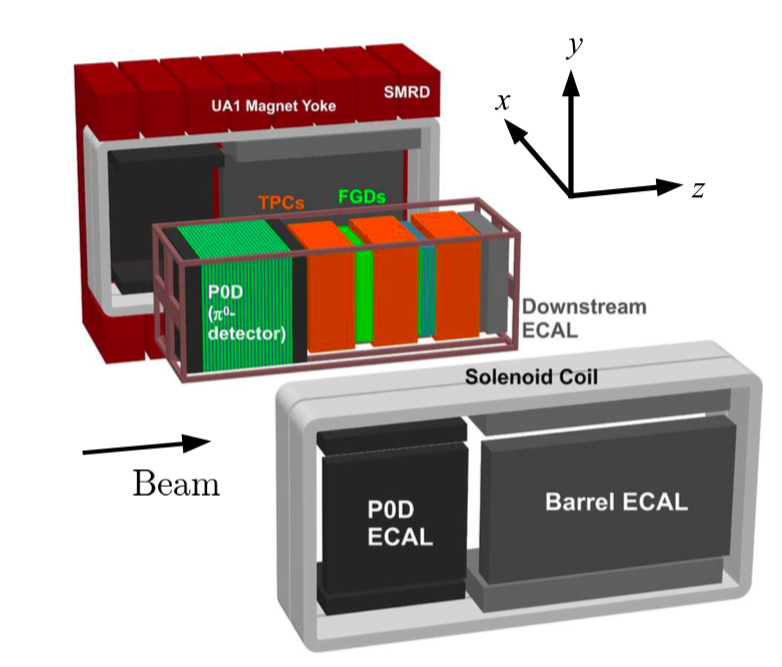
\includegraphics[width = 0.7\linewidth]{ND280}
    \caption{An exploded view of the ND280 off-axis detector.}
    \label{fig:ND280}
    \end{center}
\end{figure}

The HNL can be produced in mesons decay
\begin{equation}
    H\to\ell_ lN,
\end{equation}
where $H$ is a parent meson, $\ell$ is a lepton, $l=e,\mu, \tau$. In the T2K experiment mainly pions and kaons are produced in the proton collisions at the target station. We will focus at the kaon decay as it allows to study wide range of the HNL mass. In the T2K at the moment there is no simulation for the hadrons heavier than kaons. The decay channels of the HNL with $M_{HNL}<M_K$ are:
\begin{eqnarray}
    \label{eq:2bd}
    &N\to\ell\pi &\\
    \label{eq:3bd}
    &N\to\ell\ell\nu & \\
    &N\to\gamma\nu, \hspace{2cm}   N\to3\nu, \hspace{2cm} N\to\nu\pi^0&
    \label{eq:no}
\end{eqnarray}


We will study 2-body decays (\ref{eq:2bd}) and 3-body decays (\ref{eq:3bd}). Daughter particles from decays \ref{eq:no} are practically undetectable. The Fig.~\ref{fig:KaonMasReg} shows reactions of the HNL production and decay, that we are going to study and HNL mass region for each process.
\begin{figure}[H]
    \begin{center}
    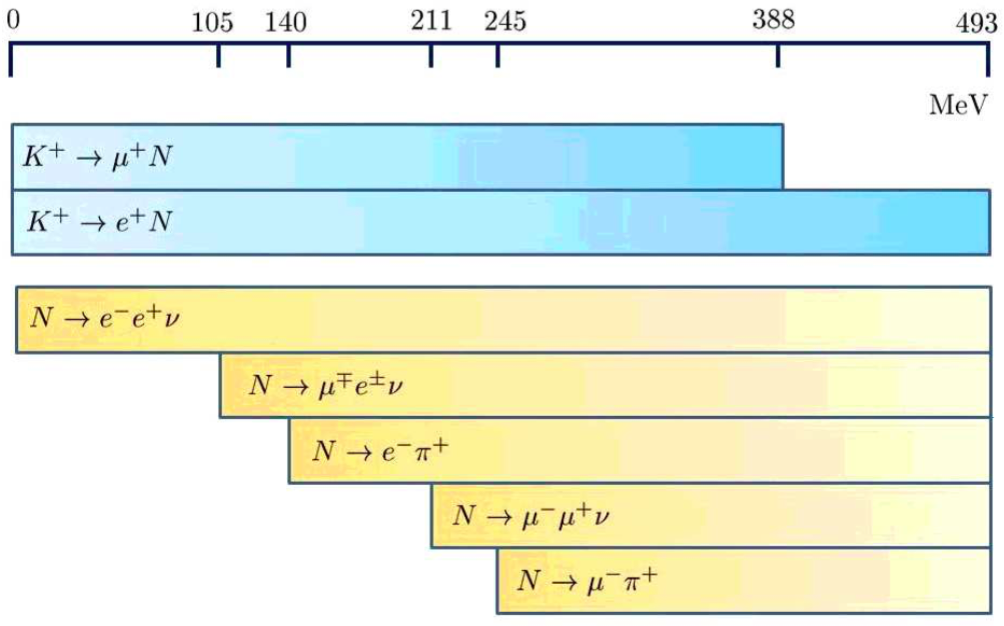
\includegraphics[width = \linewidth]{KaonMasReg}
    \caption{Summary of the production and the detection processes of the heavy neutrino. The horizontal axis corresponds to the HNL mass.}
    \label{fig:KaonMasReg}
    \end{center}
\end{figure}

It is interesting to study a dimuon decay mode of the HNL: $N\to\mu\mu\nu$. This decay has charge and neutral current contributions shown in Fig.~\ref{fig:DimuonFeynman} (from~\cite{johnson1997extending}).

\begin{figure}[H]
    \begin{minipage}[h]{0.49\linewidth}
        \center{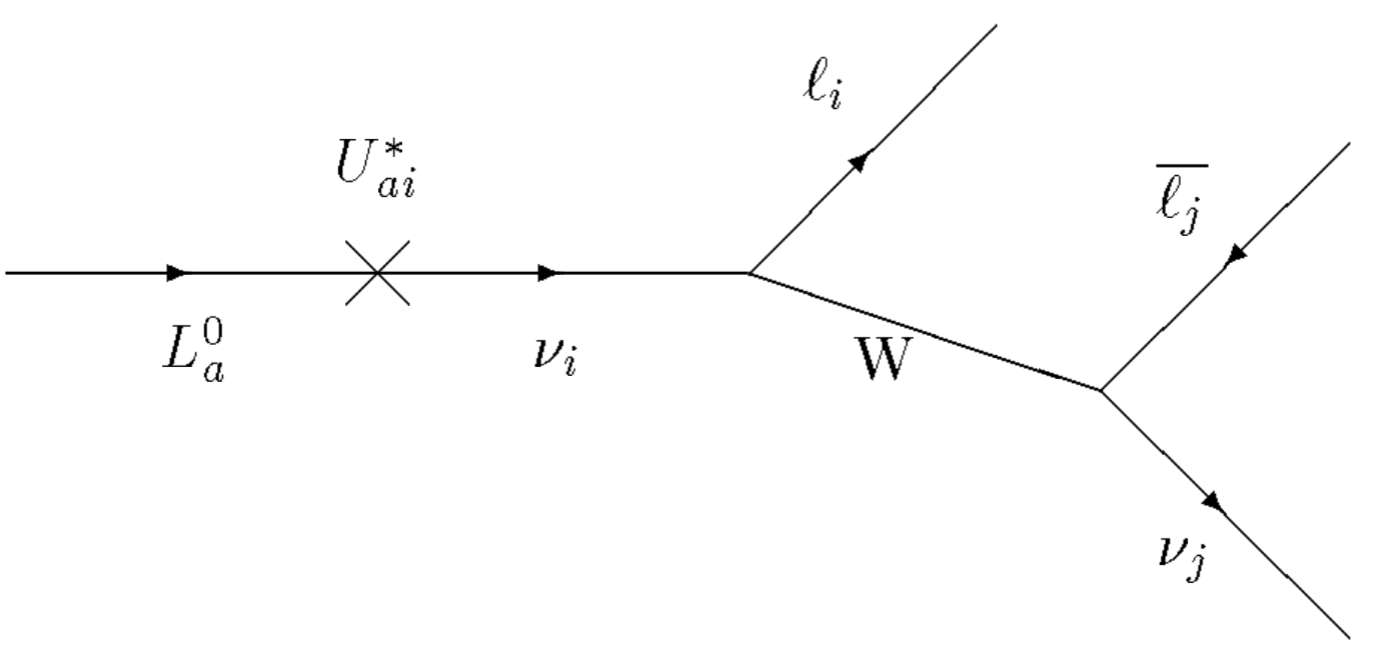
\includegraphics[width=\linewidth]{DiMuonCC} \\ a) }
    \end{minipage}
    \hfill
    \begin{minipage}[h]{0.49\linewidth}
        \center{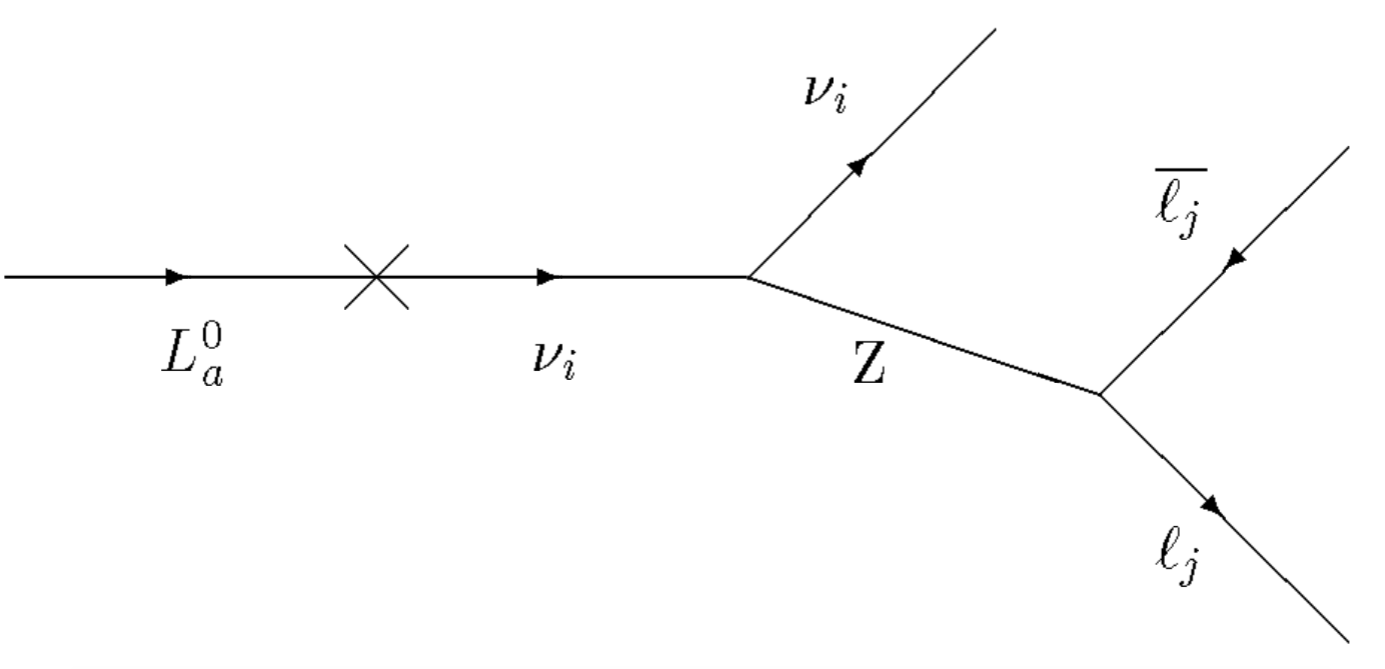
\includegraphics[width=\linewidth]{DiMuonNC} \\ b)}
    \end{minipage}
    \caption{Feynman diagrams for the HNL decay $N\to\mu\mu\nu$ via charged (a) and neutral (b) current.}
    \label{fig:DimuonFeynman}
\end{figure}

As one can see if the HNL decay via NC, any type of the active neutrino can be produced ($\nu_{e}, \nu_{\mu}, \nu_{\tau}$), so we can study the mixing element including $|U\tau|$. This is interesting as the upper limits on this element are rather high.

The T2K experiment uses neutrino beam from $\pi^\pm$ and $K^\pm$ decays. In our study a search of HNL from both $K^+$ and $K^-$ decays is carried out in order to increase sensitivity because of larger statistics. We assume the Majorana nature of a HNL, this allows to study decays of $K^+$, $K^-$ and both decay modes of a heavy neutrino to $\ell^{\pm}\pi^{\mp}$.

As we focus on search of the HNL decay there are two analysis methods:
\begin{itemize}
  \item search for a peak in the HNL candidate invariant mass spectrum
  \item search for a rare event in a low background environment
\end{itemize}

The first one requires applying some simple cuts and then study difference between data and MC estimation with a peak shape. We need a rather accurate background prediction for this method. Also invariant mass resolution is one of the most important issue. We have studied the possible resolution for the HNL signal samples. The ePvents that pass all the cuts described in the section~\ref{sec:Ana} give as the reconstructed mass distribution. The examples of such distribution are presented in Fig.~\ref{fig:InvMass}. The resolution of the invariant mass reconstruction on the HNL mass is shown in Fig.~\ref{fig:InvMassPlot}. As one can see, RMS is quite large $\approx70MeV$. The main background processes for the HNL decay are  interactions of the active neutrinos. In near detector there are three TPCs filled with argon gas. The cross sections of the neutrino interactions in gas are not studied well. Studies of these events were performed by ArgoNeuT group~\cite{acciarri2014measurements}. In our momentum region ($\approx1GeV$) the uncertainties are really large. Other background processes can be $K^0, \Lambda, \eta$ decays, deep inelastic neutrino scattering, etc. (Sec~\ref{sec:bg}) that are also poorly studied. Because of this we can not provide needed accuracy of the background prediction and the method of the invariant mass peak search can not be applied.
\begin{figure}[H]
    \begin{minipage}[h]{0.49\linewidth}
        \center{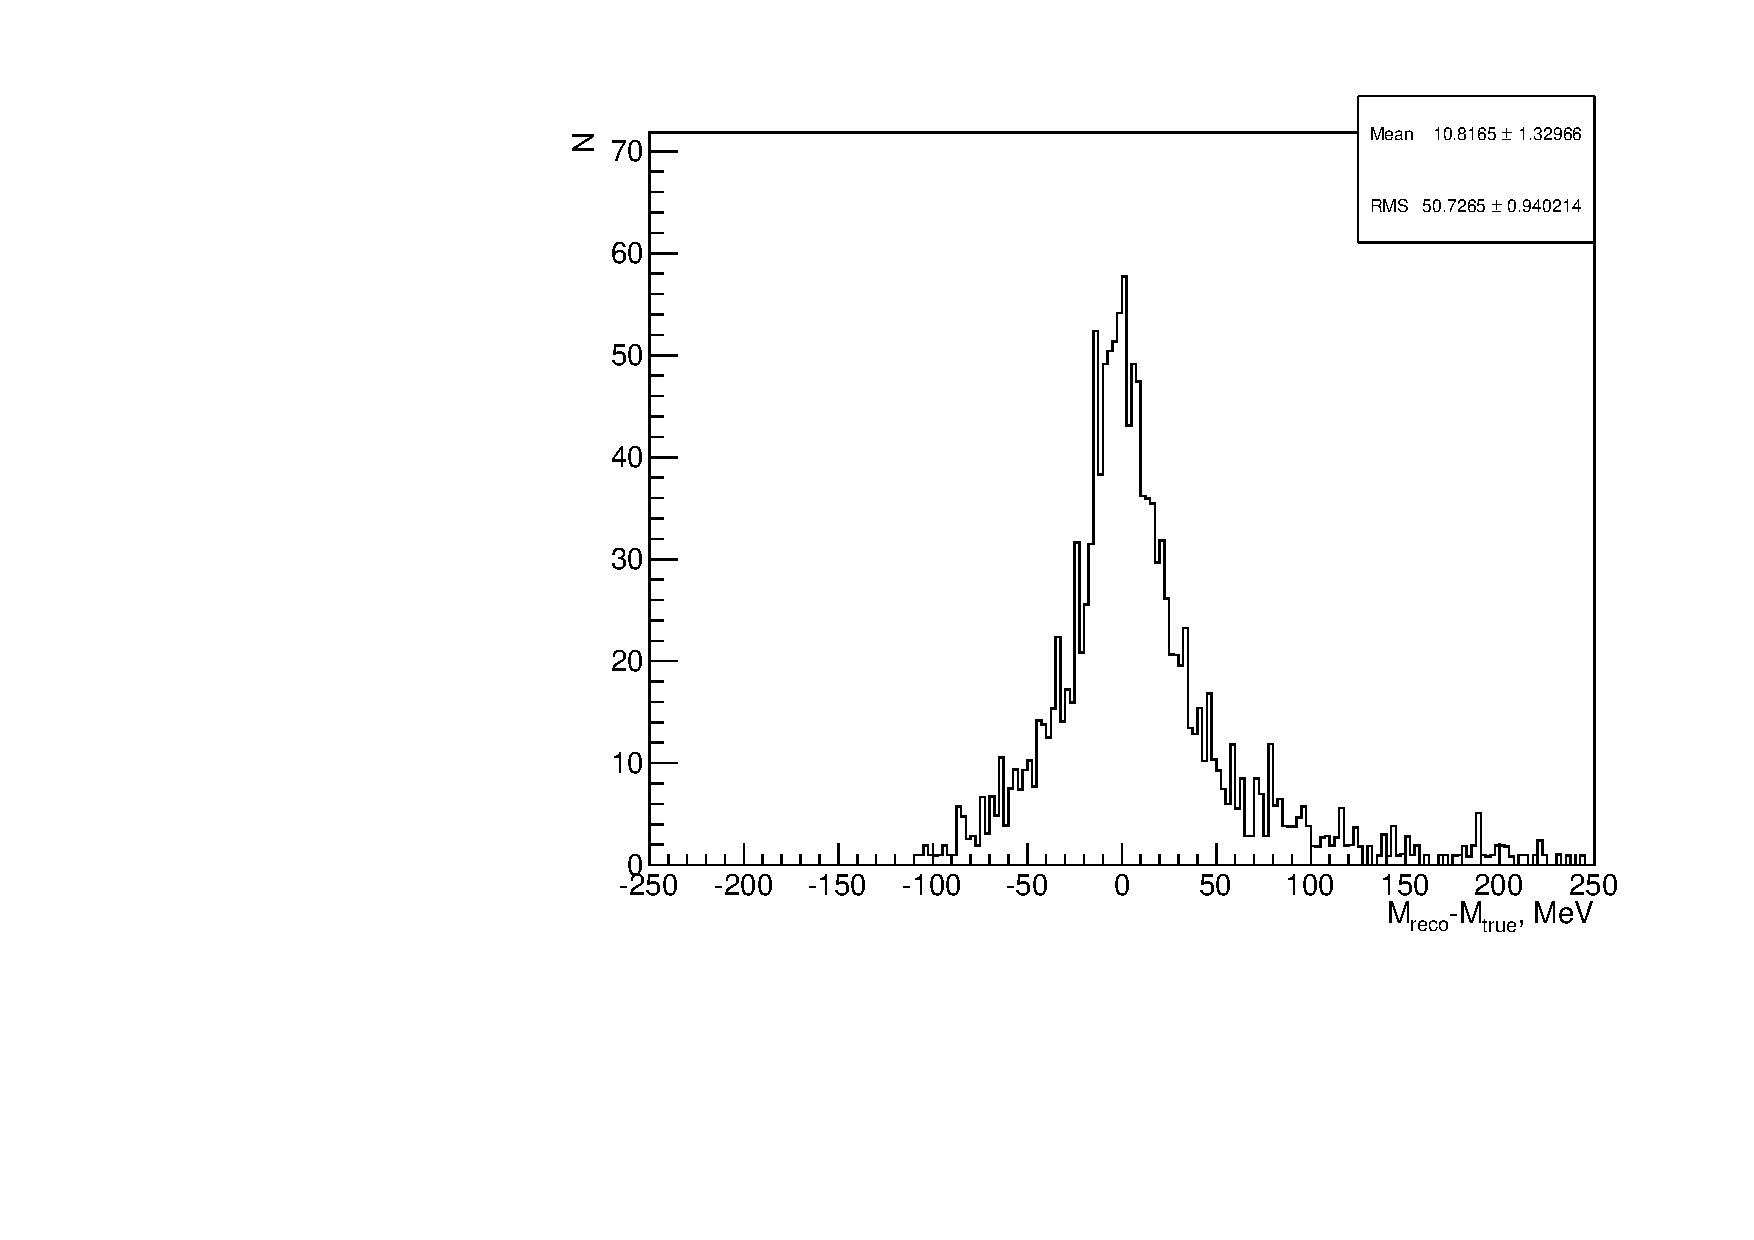
\includegraphics[width=\linewidth]{InvMass036}}
    \end{minipage}
    \hfill
    \begin{minipage}[h]{0.49\linewidth}
        \center{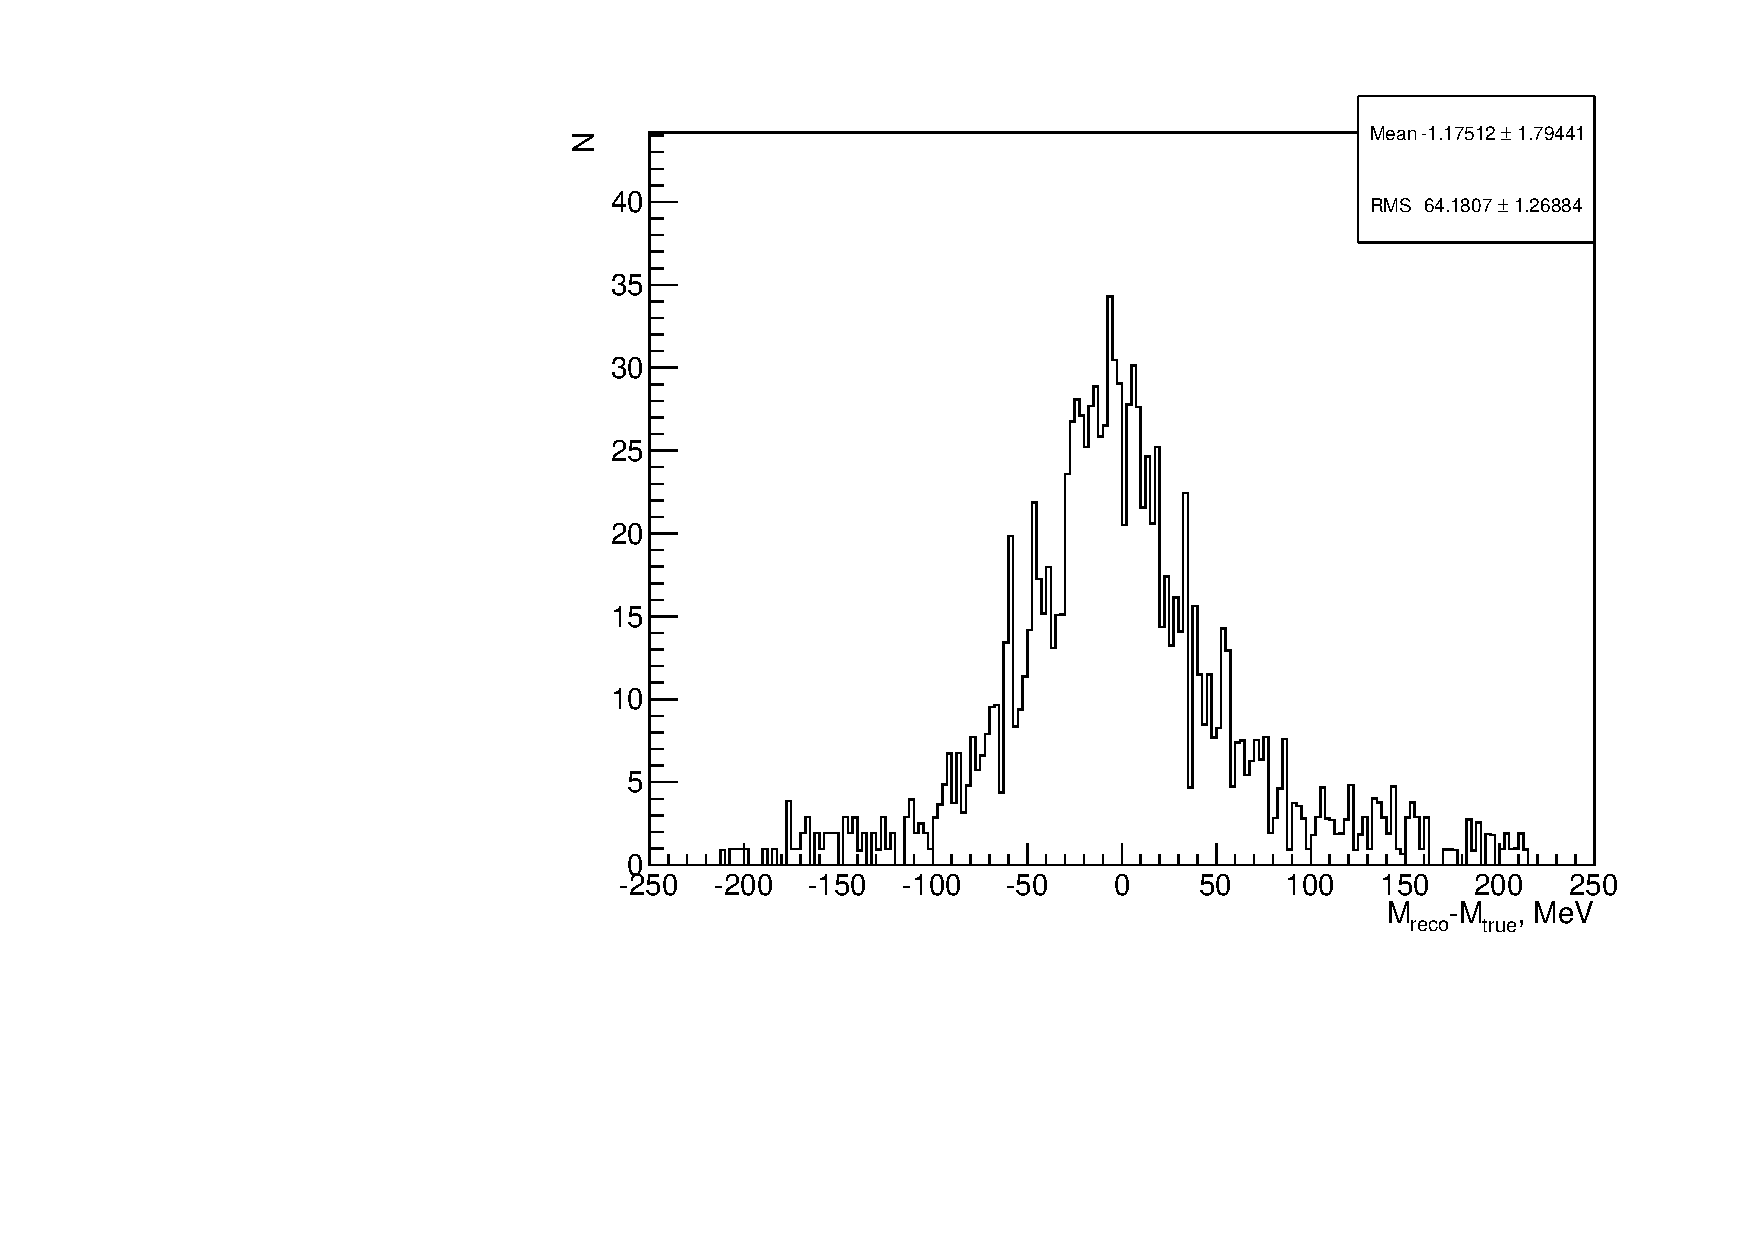
\includegraphics[width=\linewidth]{InvMass048}}
    \end{minipage}
    \caption{HNL invariant mass resolution. Left is for $M_{HNL}=360$ MeV, right is for $M_{HNL}=480$ MeV for the $\mu\pi$ mode.}
    \label{fig:InvMass}
\end{figure}

\begin{figure}[H]
    \begin{minipage}[h]{0.49\linewidth}
        \center{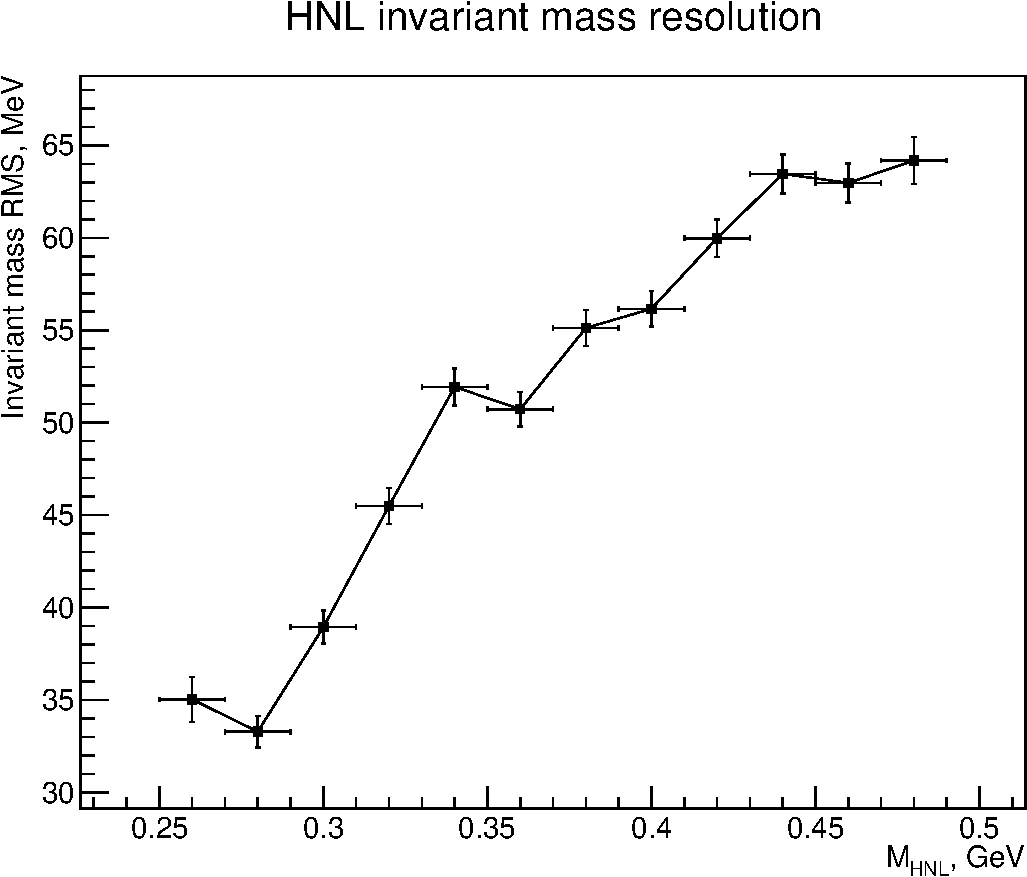
\includegraphics[width=\linewidth]{InvMassMuPlot} \\ a)}
    \end{minipage}
    \hfill
    \begin{minipage}[h]{0.49\linewidth}
        \center{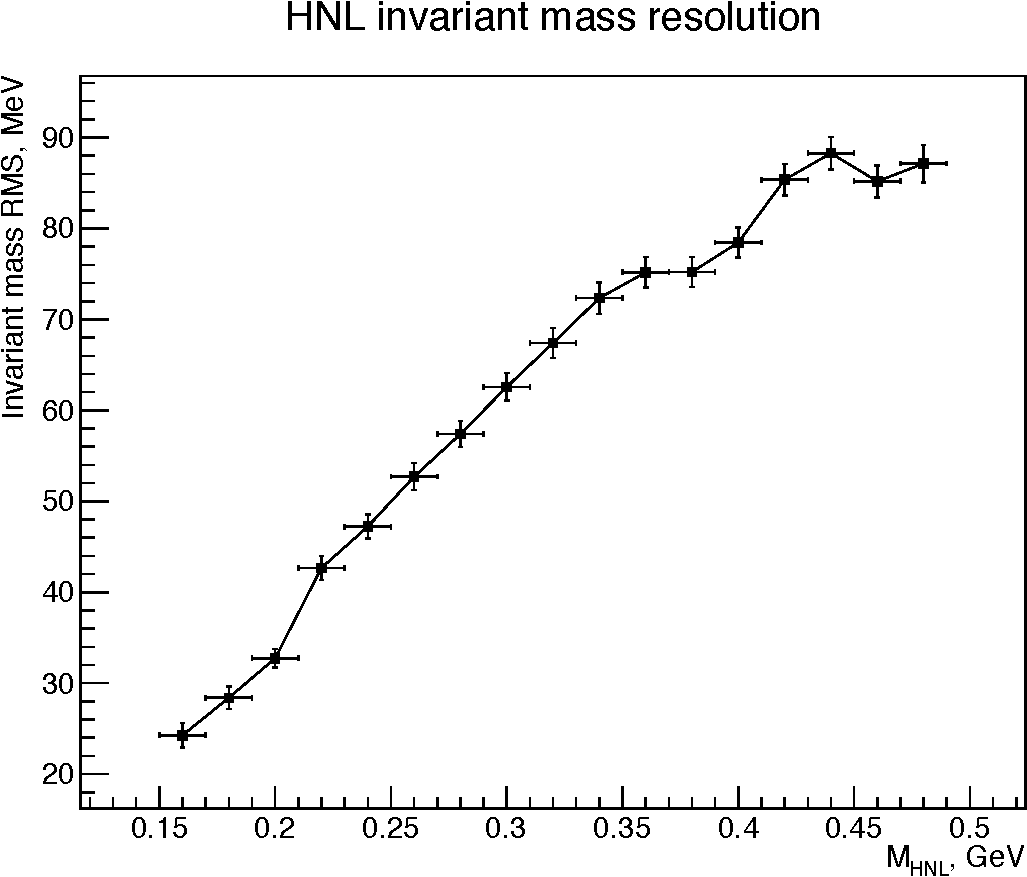
\includegraphics[width=\linewidth]{InvMassElePlot} \\ b) }
    \end{minipage}
    \caption{HNL invariant mass resolution (RMS) dependence on the HNL mass for (a) $N\to \mu\pi$ mode and (b) $N\to e\pi$ mode.}
    \label{fig:InvMassPlot}
\end{figure}

The second method requires the cut sequence for the background elimination. Then we can use low signal statistical approach which is described in Sec.~\ref{sec:LowSignal}. For background suppression we decided to use only fiducial volume of the TPCs. The difference of the density between the gas (TPC) and the scintillator (FGD) is large. As number of the active neutrino interactions depends on density, this method provides significant background reduction.

As described, the cross-section uncertainties of the active neutrino interactions in gas are large. Because of this, we are going to treat all the events that survive after all cuts applied as signal and put the constraints on mixing elements. The details of this approach is described in the next section.

\subsection{Low level signal analysis}
\label{sec:LowSignal}

The statistical approach to the low level signal analysis is described in the Highland and Cousins work~\cite{cousins1992incorporating}. As number of the HNL decay events is proportional to the forth power of the mixing element, constraints on $\left|U_i\right|^2$ without systematics looks like:
\begin{equation}
  \left|U_i\right|^2_{limit}=\sqrt{\frac{U_n}{N_{events}}}
  \label{eq:constraints}
\end{equation}
where $i=e,\mu$, $U_n$ is 90\% C.L. Poisson limit for $n$ observed events and $N_{events}$ is expected number of signal events assuming $\left|U\right|^2=1$. If we take into account the detector acceptance uncertainty, the result can be calculated according to Ref.~\cite{cousins1992incorporating}:
\begin{equation}
  U_n=U_{n0}\left\{1+E_n\frac{\sigma^2_{Acc}}{2}\left(1+\left(\frac{E_n\sigma_{Acc}}{2}\right)^2\right)\right\}
  \label{eq:constrainsAcc}
\end{equation}
where $U_{n0}$ is 90\% C.L. Poisson limit for $n$ observed events, $\sigma_{Acc}$ is the acceptance error, $E_n=U_{n0}-n$ represents the excess of the upper limit of
a Poisson parameter over the number n of observed events, for a specified confidence level. This approach can be applied only while $\sigma_{Acc}<1/E_n$. We will show that in our study $\sigma_{Acc}\approx0.3$ and $1/E_n>0.5$ (this values are described in the section~\ref{sec:syst}). So this method can be applied for the analysis.
\end{comment}




\chapter{HNL flux simulations}
\section{T2K flux simulation}
\section{HNL production}
\section{HNL decays}
\chapter{Analysis}
\section{Event selection}
\subsection{Signal event selection}
\subsection{Background suppression}
\section{Systematic uncertainties}
\subsection{Detector systematics}
\subsection{Flux systematics}
\subsection{Pile up}
\section{Statistical methods}
\chapter{Results}
\section{MC sensitivity estimations}
\section{Data unbinding}
\end{document}